\documentclass[10pt,pdf,hyperref={unicode}, dvipsnames]{beamer}
\usepackage[english,russian]{babel}
% \usepackage[T2A,T1]{fontenc}
\usepackage[utf8]{inputenc}
\usepackage{tikz}
\usepackage[unicode]{hyperref}
\usepackage{pgfplots,standalone}
\usepackage{caption}
\usepackage[normalem]{ulem}
\usepackage
	{
		% Дополнения Американского математического общества (AMS)
		amssymb,
		amsfonts,
		amsmath,
		amsthm,
		physics
		}
% \usepackage{lmodern}
\pgfplotsset{compat=newest} 
\usetikzlibrary{%
    decorations.pathreplacing,%
    decorations.pathmorphing,%
    patterns,%
    angles,%
    quotes,%
    calc, %
    3d, %
    backgrounds, %
    positioning%
}


% Стиль презентации

 \usetheme{default}
 \usefonttheme{professionalfonts}
 \usecolortheme{}
 % \usecolortheme{whale}
% \let\oldframe\enumerate
% \renewcommand{\frame}{%
% \oldframe
% \let\olditemize\itemize
% \renewcommand\itemize{\olditemize\addtolength{\itemsep}{100pt}}%
% }
 

% \setbeamercolor{frametitle right}{fg=white,bg=Brown!85}
% \setbeamercolor{frametitle}{fg=white,bg=Brown!85}
%\setbeamercolor{frametitle right}{fg=white,bg=black!85} %
\definecolor{MyBG}{RGB}{46,47,114}
%\setbeamercolor{frametitle}{fg=white,bg=black!85} % Цвет титульника
\setbeamercolor{frametitle}{fg=white,bg=MyBG}

\setbeamercolor{item projected}{fg=white,bg=MyBG} % Цвет титульника
\setbeamertemplate{blocks}[rounded][shadow=false] %стиль блоков
\setbeamertemplate{itemize item}{\color{MyBG}$\bullet$}
\setbeamertemplate{headline}{}
\setbeamertemplate{footline}{} 
\setbeamertemplate{navigation symbols}{} % минус навигация
\let\Tiny=\tiny % решает проблему со шрифтами в TexLive
%\setbeamertemplate
%	{footline}{
%		\color{black!40!white}
%		\quad\hfill
%		\insertframenumber/\inserttotalframenumber
%		\hfill\vspace{1cm}\quad
%	} 


\beamersetrightmargin{1cm} 
\beamersetleftmargin{1cm}

\setbeamertemplate{enumerate item}{
	\usebeamercolor[bg]{item projected}
	\raisebox{1pt}{\colorbox{MyBG}{\color{fg}\footnotesize\insertenumlabel}}%
}

% \setbeamertemplate{itemize item}{%
% 	\usebeamercolor[bg]{item projected}%
% 	\raisebox{3pt}{{\colorbox{black!85}\footnotesize$\bf$\bullet}}%
% }

\setbeamercolor{item projected}{bg=black,fg=white}
\setbeamercolor{title}{bg=MyBG,fg=white}

\setbeamertemplate{frametitle}
{	
	\nointerlineskip
	\begin{beamercolorbox}[sep=15pt,ht=1.9em,wd=\paperwidth]{frametitle}
		\vbox{}\vskip-15pt%
		\strut\insertframetitle\strut
		\vskip-12pt%	
	\end{beamercolorbox}
}
\renewcommand{\phi}{\varphi}
\renewcommand{\epsilon}{\varepsilon}
\renewcommand{\div}{\operatorname{div}}
\title[Метод молекулярно-пучковой эпитаксии]{Метод молекулярно-пучковой эпитаксии}
%\tolerance-1
\hyphenpenalty=10000 %минус переносы

%\usefonttheme{serif}
%\usepackage{helvet}
%\setmainfont{Helvetica}


\author{% 
\large Виноградов И.Д. %
	Понур К.А. %
	Шиков А.П. %
}

\institute{Радиофизический факультет ННГУ, 430 группа \\ \vspace{5mm} \large Научный руководитель: Лобанов Д.Н. \normalsize \vspace{5mm}}

\date{Нижний Новгород, 2018}

\begin{document}  
\begin{frame}
\titlepage
\end{frame}


\section{Введение}
\subsection{Определение эпитаксии}
\begin{frame}[t]
	\frametitle{Определение эпитаксии}
	\textbf{Эпитаксия} - это закономерное нарастание одного кристаллического материала на другой, т.е. ориентированный
	рост одного кристалла на поверхности другого.
	\vspace{20pt}

	\centering
	\begin{minipage}{0.49\linewidth}
		\centering
		\textbf{Авто(гомо)эпитаксия}

		Материалы осаждаемого слоя и подложки идентичны
		\centering

		\includegraphics[width=0.6\linewidth]{imgs/Cell.png}
		
		Решетка германия и кремния
	\end{minipage}
	\begin{minipage}{0.49\linewidth}
		\centering
		\textbf{Гетероэпитаксия}

		Материалы осаждаемого слоя и подложки различны
		%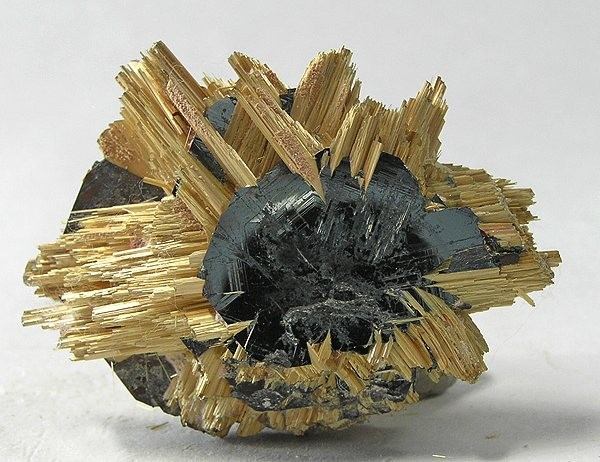
\includegraphics[width=0.9\linewidth]{imgs/RutHem.jpg}
		%Рутил на гематите
	\end{minipage}

\end{frame}


\subsection{Область применения}
\begin{frame}[t]
	\frametitle{Область применения}
	Эпитаксия является одним из базовых процессов технологии изготовления полупроводниковых приборов и интегральных
	схем.
	\vspace{20pt}

	Преимущества эпитаксиальной технологии
	\begin{enumerate}
		\item Широкая область изменения уровня и профиля легирования 
		\item Возможность изменения типа проводимости выращиваемых эпитаксиальных слоев
		\item Возможность проведения роста при температурах меньших, чем температура роста монокристалла
		\item Возможность нанесения слоя как на большие площади, так и локально
		\item Рост соединений со сложным, контролируемым составом
	\end{enumerate}

\end{frame}



\section{Методы эпитаксиального роста}
\subsection{Методы эпитаксиального роста}
\begin{frame}[t]
	\frametitle{Методы эпитаксиального роста}
	% Существует три основных метода эпитаксиального роста: \textit{Жидкофазная}, \textit{газофазная} и
	% \textit{молекулярно-пучковая} эпитаксия.

	Жидкофазная: Монокристаллические слои получают из контактирующей с подложкой перенасыщенных жидких растворов.

	\textbf{Недостатки}: Сложности контроля параметров получаемых пленок, низкое качество. 
	\vspace{8pt}

	Газофазная: Вещество, необходимое для роста поступает к подложке в составе химического соединения, с выделением при
	разложении вещества, необходимого для роста эпитаксиальной пленки.

	\textbf{Достоинства}: Высокая скорость роста, высокая производительность.

	\textbf{Недостатки}: Токсичность, зависимость скорости роста от температуры подложки.
	\vspace{8pt}

	Молекулярно-лучевая: Хим. элементы, необходимые для роста поступают на подложку в виде молекулярных пучков этих
	элементов.
	
	\textbf{Достоинства}: Возможность роста при пониженных температурах, лучший по сравнению с ГФЭ контроль над составом и
	толщиной слоев.

	\textbf{Недостатки}: Низкая производительность, дороговизна(необходим сверхвакуум).
\end{frame}

\section{Основы МПЭ}
\subsection{Гетероэпитаксиальный рост}
\begin{frame}[t]
	\frametitle{Механизмы гетероэпитаксиального роста}
	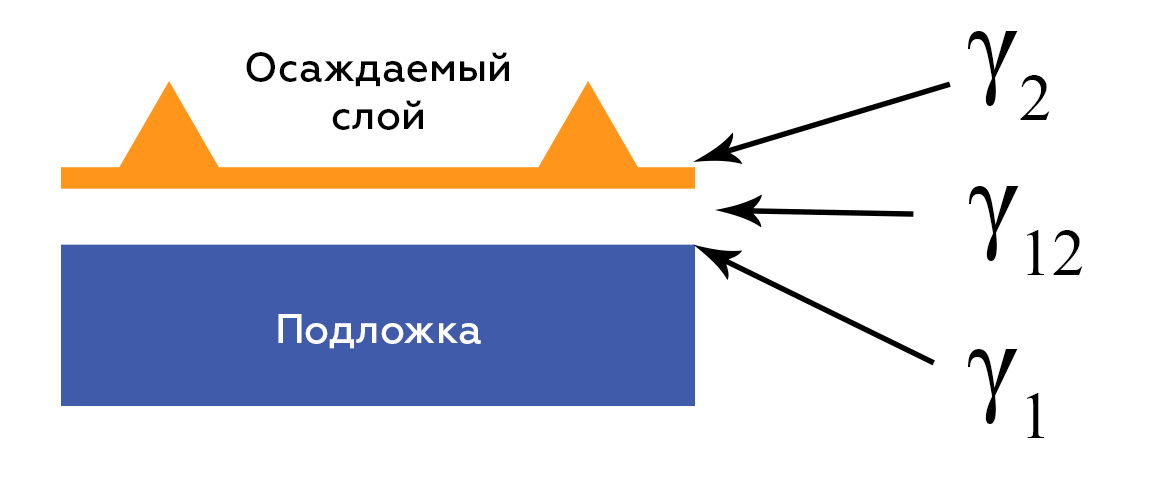
\includegraphics[width = \linewidth]{imgs/struct.png}
	\Large

	$\gamma_1$ - Энергия поверхности подложки
	
	
	$\gamma_{12}$ - Энергия границы раздела
	
	
	$\gamma_2$ - Энергия поверхности осаждаемого материала


\end{frame}

\normalsize
\begin{frame}[t]
	\frametitle{Механизмы гетероэпитаксиального роста}
	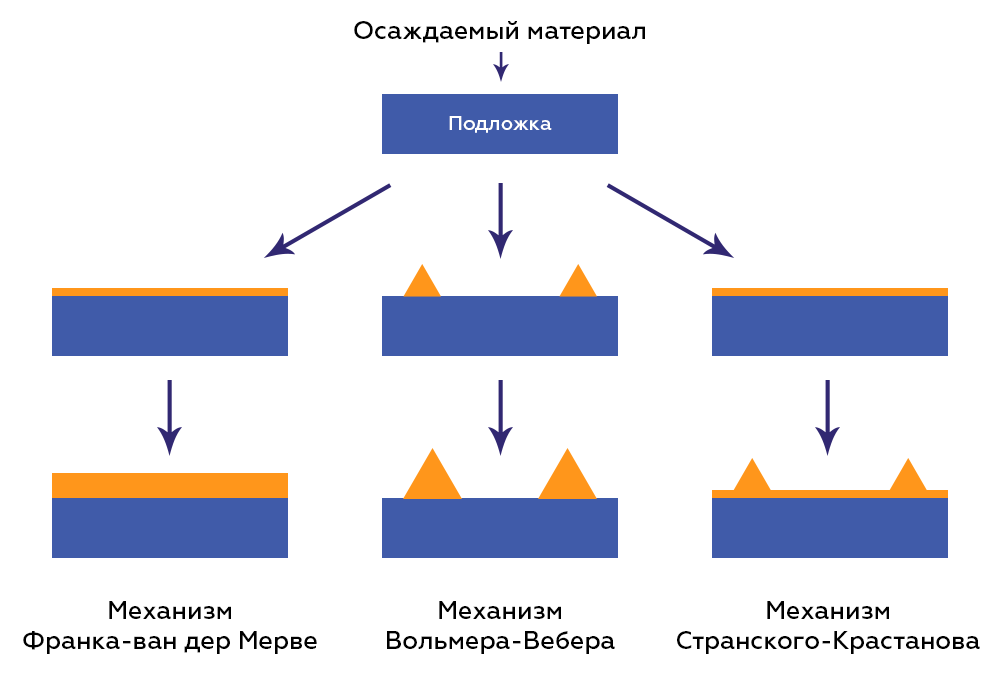
\includegraphics[width = \linewidth]{imgs/growth.png}

	\centering
	\begin{minipage}{0.32\linewidth}
		\centering
		$ \gamma_2+\gamma_{12}<\gamma_1 $	
	\end{minipage}
	\begin{minipage}{0.32\linewidth}
		\centering
		$ \gamma_2+\gamma_{12}>\gamma_1 $	
	\end{minipage}
	\begin{minipage}{0.32\linewidth}
		\centering
		Подробнее далее %Как по мне лучше оставить формулу
	\end{minipage}

\end{frame}

\subsection{Механизм Странского-Крастанова}
\begin{frame}[t]
	\frametitle{Механизм Странского-Крастанова}
	\begin{minipage}{0.4\linewidth}
		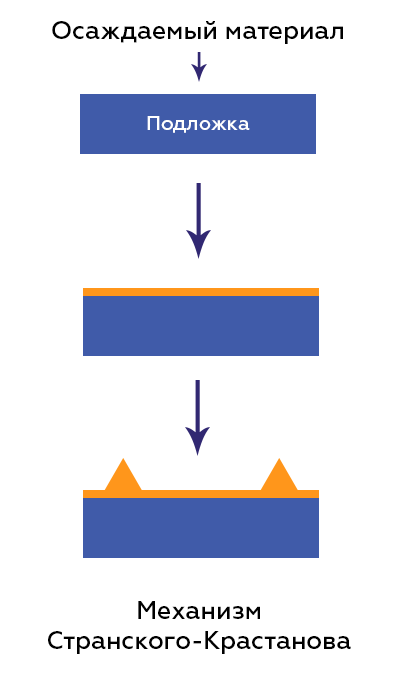
\includegraphics[width = \linewidth]{imgs/SKM.png}
	\end{minipage}	
	\begin{minipage}{0.59\linewidth}
		Такой механизм имеет место, когда межатомное расстояние в решетке осаждаемого материала и в решетке подложки
		имеют рассогласования.

		На начальных этапах выполняется $$ \gamma_2+\gamma_{12}<\gamma_1 $$ и образуется <<смачивающий>>   слой, приводящий к уменьшению суммарной энергии системы. С определенной
		толщины энергия упругих напряжений увеличивается, увеличивая общую энергию системы, из-за чего происходит релаксация упругой энергии.
	\end{minipage}
\end{frame}

\subsection{Релаксация упругих напряжений}
\begin{frame}[t]
	\vfill
	\frametitle{Механизмы релаксации упругих напряжений}
	\centering
	\begin{minipage}{0.15\linewidth}
		\vfill
		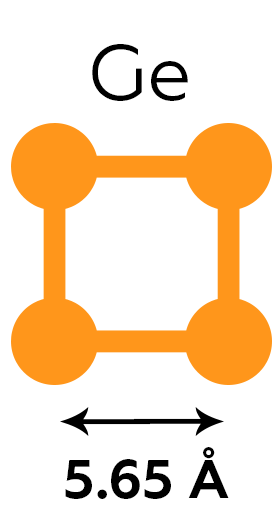
\includegraphics[width=\linewidth]{imgs/Gecell.png}
		\vfill

		\includegraphics[width=\linewidth]{imgs/Sicell.png}
		\vfill
	\end{minipage}
	\begin{minipage}{0.84\linewidth}
	\centering
		
		<<Классический>> рост по механизму Странского-Крастанова
		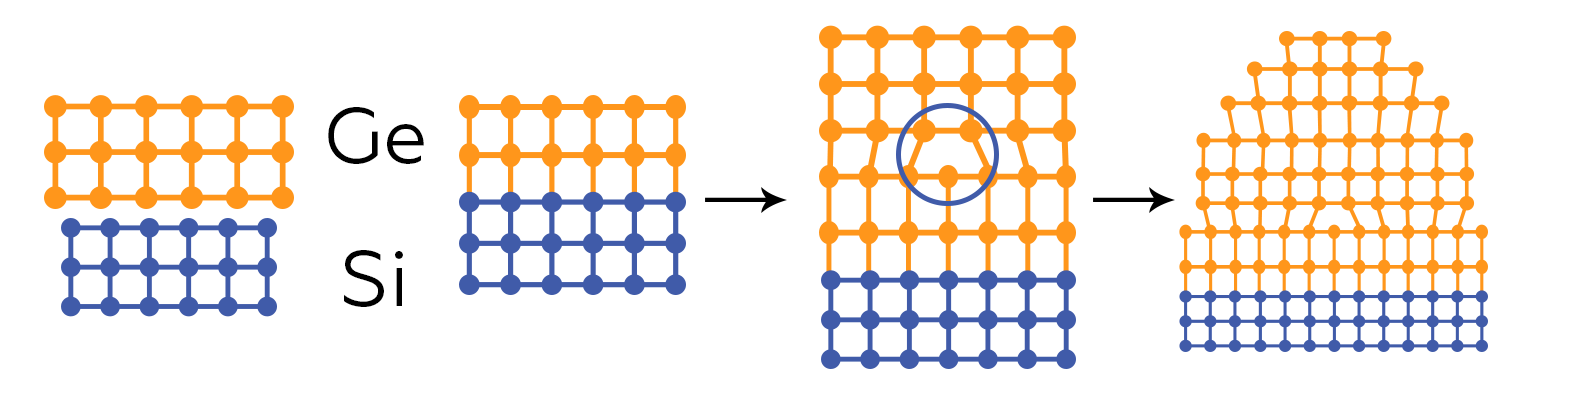
\includegraphics[width = \linewidth]{imgs/11st.png}
		
		<<Когерентный>> рост по механизму Странского-Крастанова
		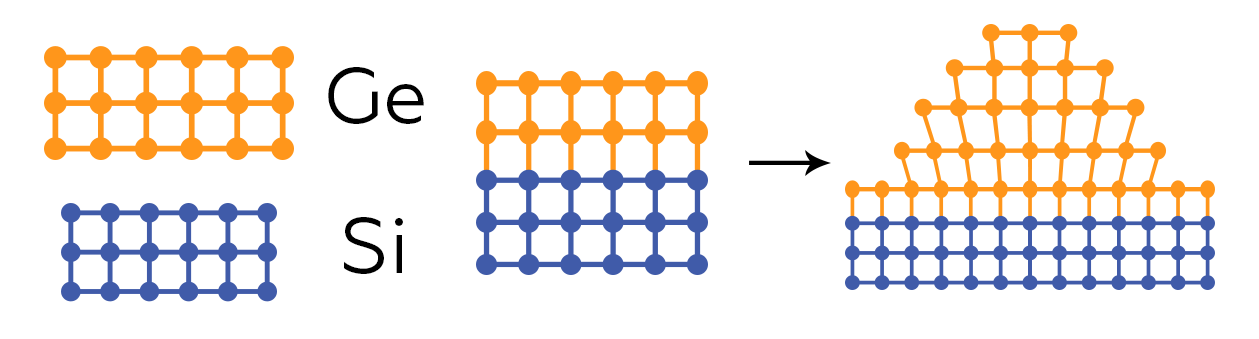
\includegraphics[width = \linewidth]{imgs/22st.png}

		$$ \Delta E_{\text{сист}} = \Delta E_{\text{упр}}+\Delta E_{\text{пов}} < 0$$
		
	\end{minipage}
	\vfill
\end{frame}

\section{Рост SiGe структур}
\subsection{Реконструкция поверхности Si}
\begin{frame}[t]
	\frametitle{Реконструкция поверхности Si(001)}
	Уменьшение энергии системы за счет реконструкции на границе.
	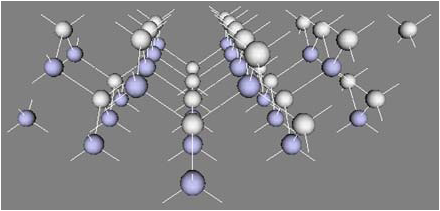
\includegraphics[width = .49\linewidth]{imgs/rec0.png}
	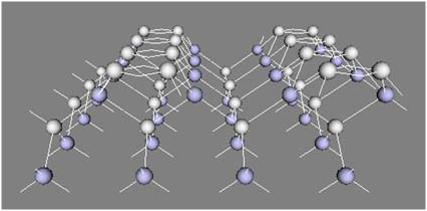
\includegraphics[width = .49\linewidth]{imgs/rec1.png}
	\centering
	\begin{minipage}{0.2\linewidth}
		\centering
		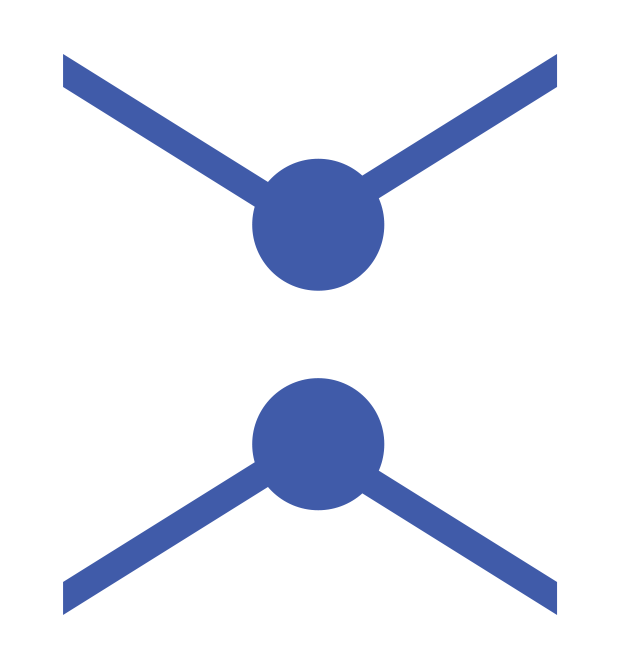
\includegraphics[width = .5\linewidth]{imgs/Dim1.png}
	\end{minipage}
	\begin{minipage}{0.79\linewidth}
		Димер - два близко расположенных атома Si
	\end{minipage}

	\begin{minipage}{0.35\linewidth}
		\centering
		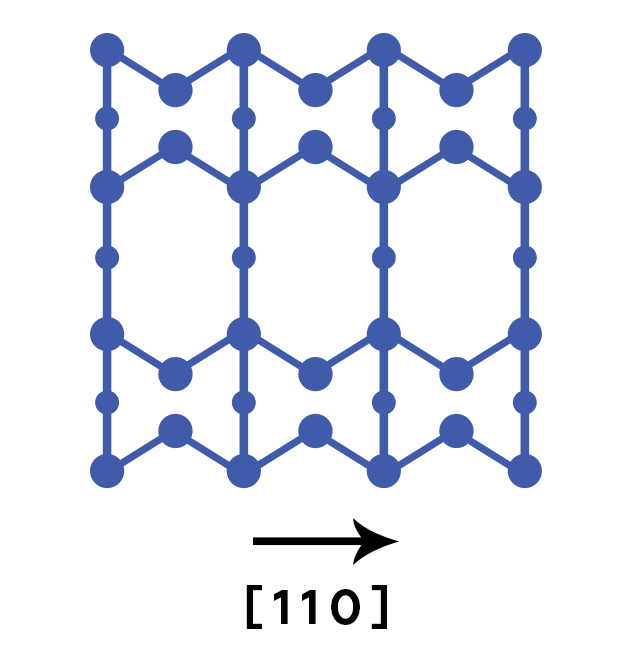
\includegraphics[width = .9\linewidth]{imgs/Dim.png}
	\end{minipage}
	\begin{minipage}{0.62\linewidth}
		Образование димеров уменьшает энергию свободных связей поверхностных атомов. Димеры выстраиваются в цепочки, 
		направление которых в каждом последующем слое меняется на 90$^\circ$
	\end{minipage}


\end{frame}

\begin{frame}[t]
	\frametitle{Реконструкция поверхности Ge на Si(001)}
	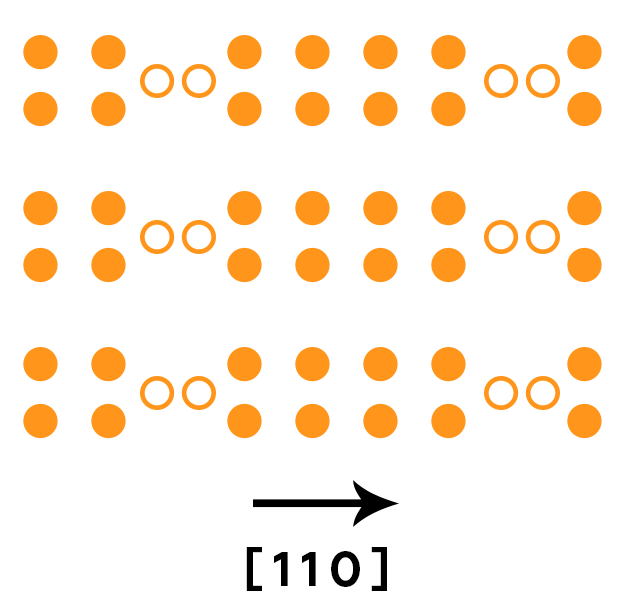
\includegraphics[width = .49\linewidth]{imgs/Dim2.png}
	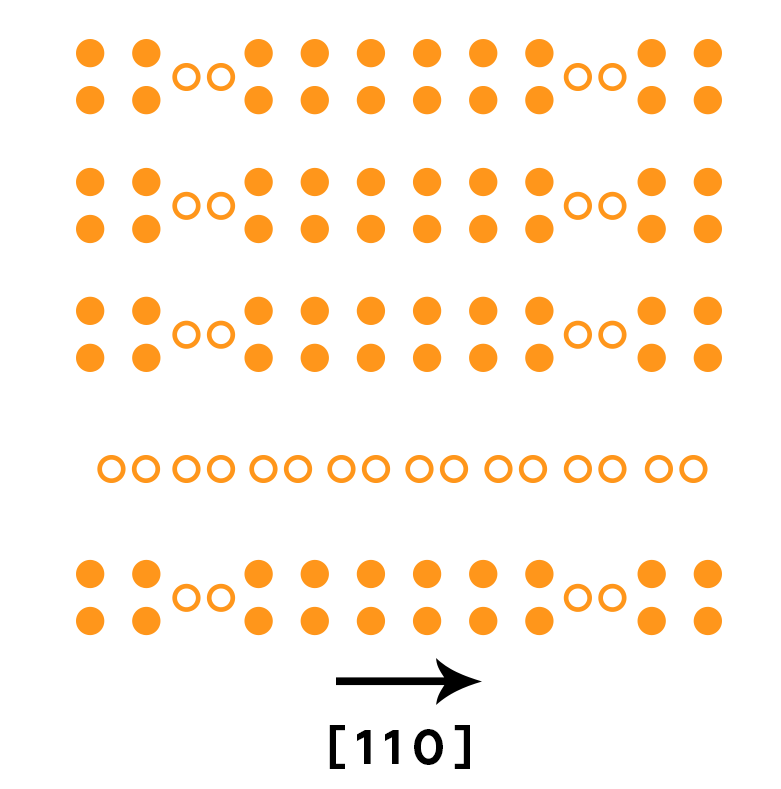
\includegraphics[width = .49\linewidth]{imgs/DimM.png}


	При росте Ge на Si, в результате рассогласования параметров решетки, пленка Ge испытывает упругие напряжения сжатия.
	Эти напряжения приводят к образованию дивакансий в цепочках димеров.	
\end{frame}

\begin{frame}[t]
	\frametitle{Релаксация за счет образования 3D - структур}
	Образования Ge островков происходит возле углублений, образованных пересечениями отсутствующих димеров.

	Толщина пленки при которой начинается формирование островков $d_{\text{кр}}$ для Ge, осаждаемого на Si(001), лежит в
	диапозоне 3-5 монослоев
	
	\centering
	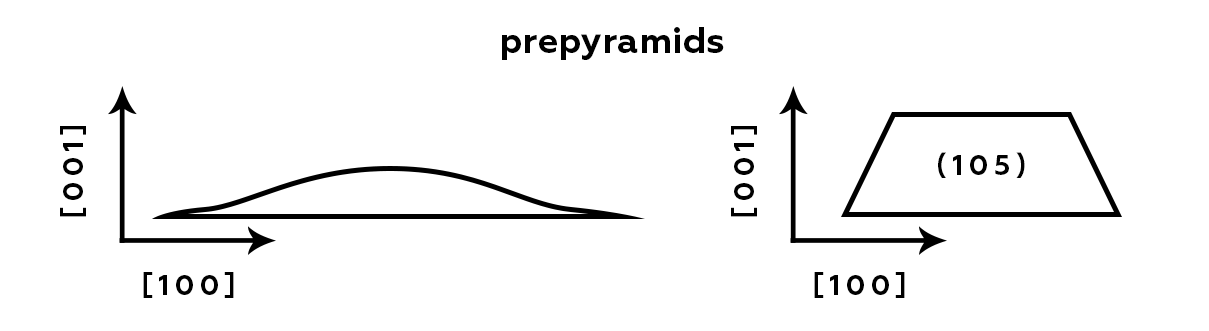
\includegraphics[width = 0.99\linewidth]{imgs/Pre.png}
	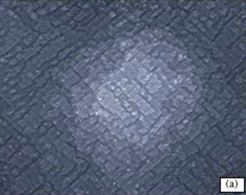
\includegraphics[width = .35\linewidth]{imgs/prepyra.jpg}
	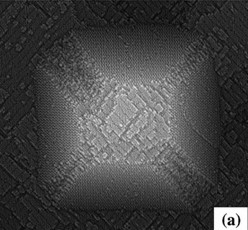
\includegraphics[width = .3\linewidth]{imgs/pyra.jpg}

	%**Принцип роста островков(см стр 16)**

\end{frame}

\begin{frame}[t]
	\frametitle{Типы образуемых островков}

	% \centering

	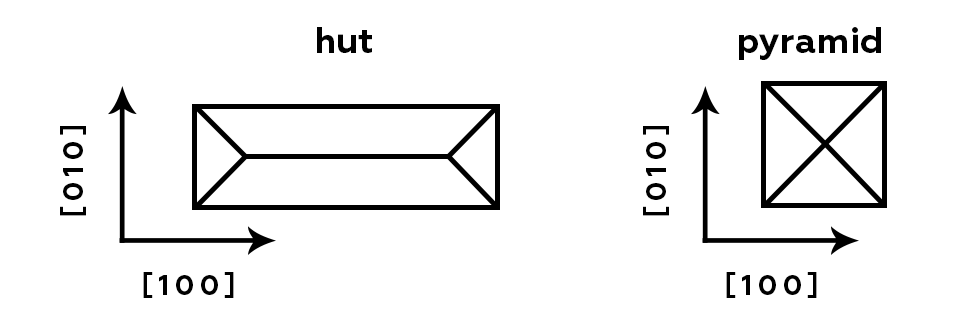
\includegraphics[width = 0.8\linewidth]{imgs/Pyr.png}

	\begin{minipage}{0.4\linewidth}
		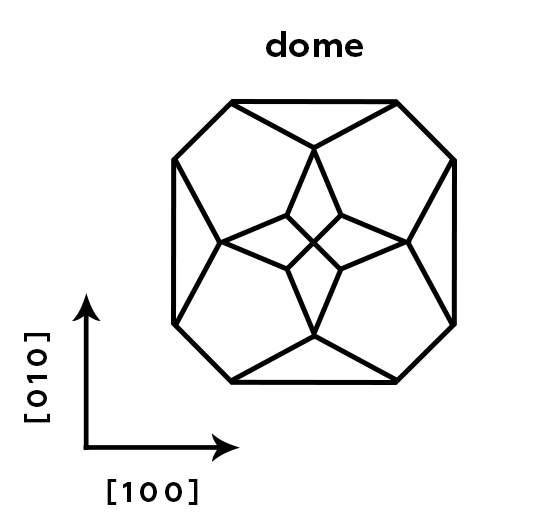
\includegraphics[width = \linewidth]{imgs/Dome.png}
	\end{minipage}
	\begin{minipage}{0.59\linewidth}
		
		$L - \text{ латеральный размер}\\ h - \text{ высота}$
		\vspace{10pt}
		
		\textbf{Hut} - островки:\\ $t_{\text{форм.}}\leq 580^{\circ}C,L: 15 - 20 \text{ нм}, h \leq 2 \text{ нм}$
		\vspace{10pt}

		\textbf{Pyramid} - островки:\\ $t_{\text{форм.}} \text{ любая}$
		\vspace{10pt}

		\textbf{Dome} - островки:\\ $t_{\text{форм.}}\geq 580^{\circ}C,L \geq 60 \text{ нм}, h \geq 10 \text{ нм}$

	\end{minipage}
	%**типы островков и условия для их образования  стр 18**
\end{frame}

\begin{frame}[t]
	\frametitle{Молекулярно-пучковая эпитаксия}
	\centering
	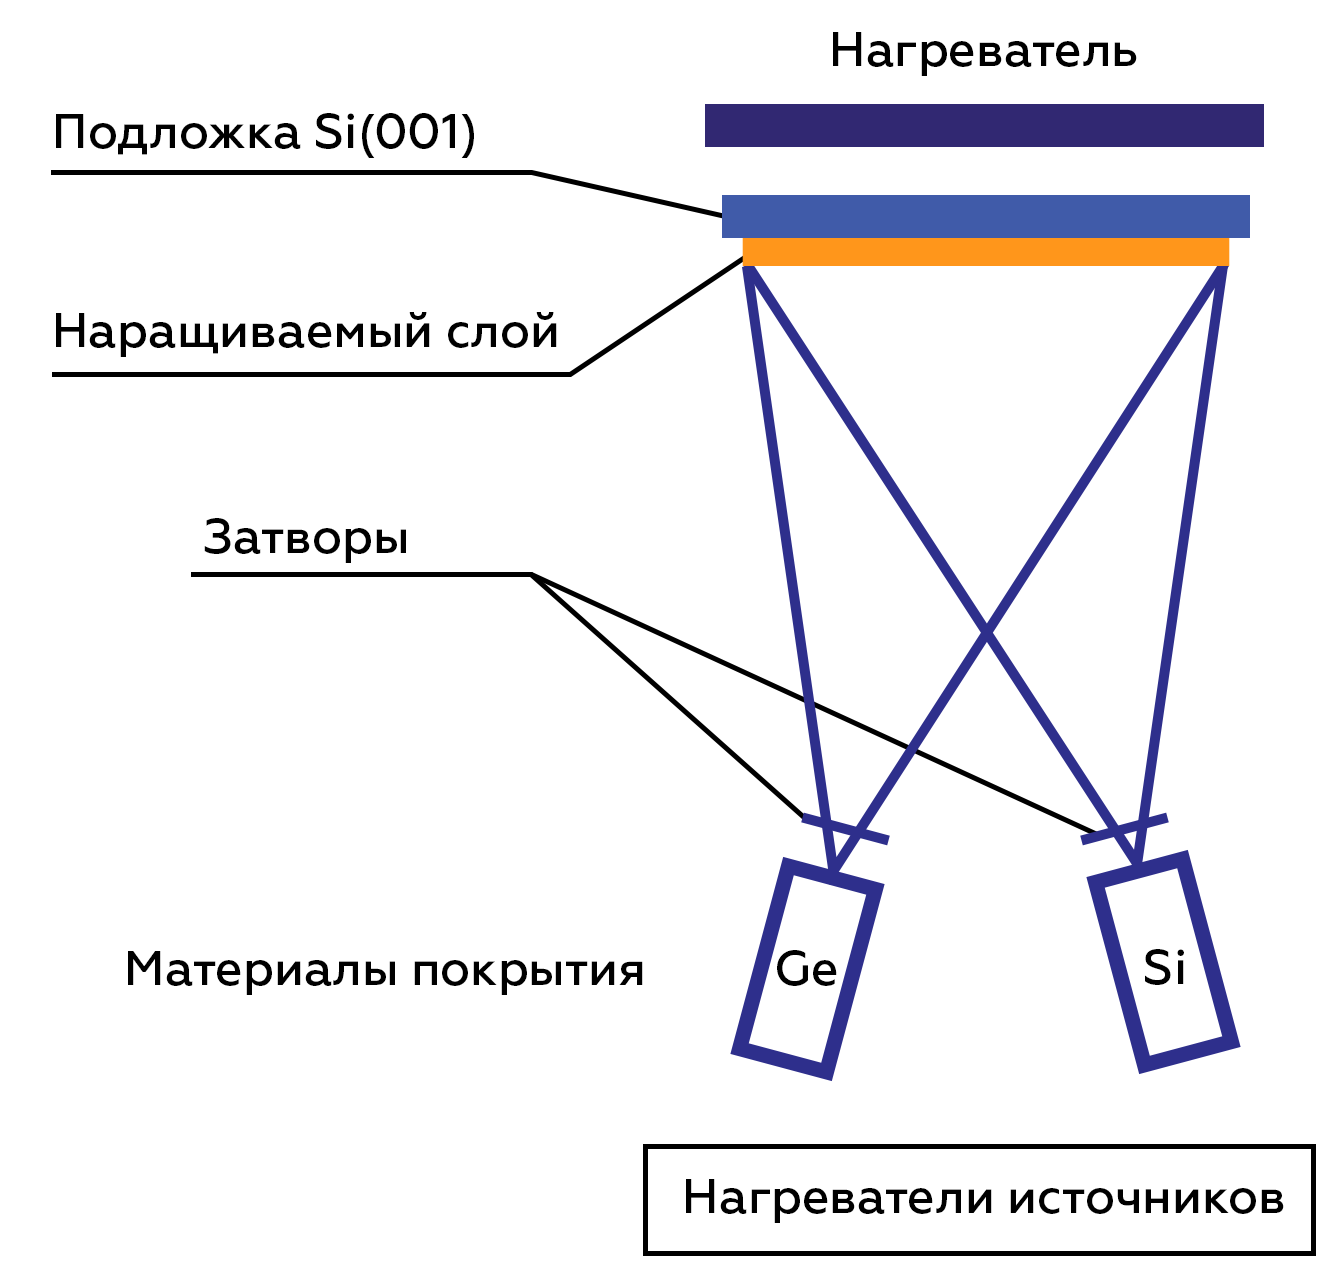
\includegraphics[width = .75\linewidth]{imgs/MBE.png}
\end{frame}


\section{Эксперимент}
\begin{frame}[t]
	\frametitle{Установка}
	\centering
	\includegraphics[width = .8\linewidth]{imgs/exp.jpg}
\end{frame}


\begin{frame}[t]
	\frametitle{Плотность поверхностного покрытия}
	\centering
	\begin{minipage}{0.32\linewidth}	
		\centering
		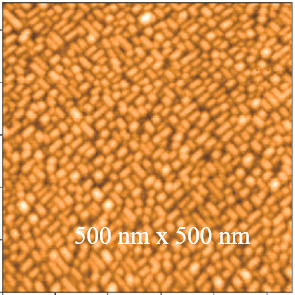
\includegraphics[width = \linewidth]{imgs/exp/460.png}
		$460^{\circ}C$	
	\end{minipage}
	\begin{minipage}{0.32\linewidth}	
		\centering
		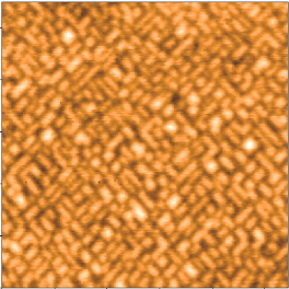
\includegraphics[width = \linewidth]{imgs/exp/500.png}
		$500^{\circ}C$	
	\end{minipage}
	\begin{minipage}{0.32\linewidth}	
		\centering
		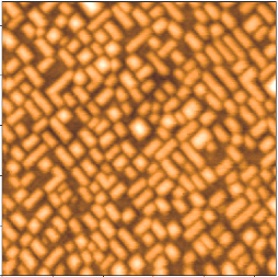
\includegraphics[width = \linewidth]{imgs/exp/550.png}
		$550^{\circ}C$	
	\end{minipage}
	\vspace{10pt}

	\begin{minipage}{0.32\linewidth}	
		\centering
		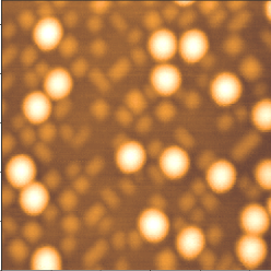
\includegraphics[width = \linewidth]{imgs/exp/580.png}
		$580^{\circ}C$	
	\end{minipage}	
	\begin{minipage}{0.32\linewidth}	
		\centering
		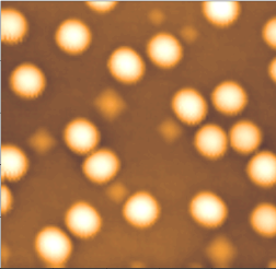
\includegraphics[width = \linewidth]{imgs/exp/600.png}
		$600^{\circ}C$	

	\end{minipage}

\end{frame}
\end{document}
